\let\negmedspace\undefined
\let\negthickspace\undefined
\documentclass[journal,12pt,twocolumn]{IEEEtran}
\usepackage{gensymb}
\usepackage{polynom}
\usepackage{amssymb}
\usepackage[cmex10]{amsmath}
\usepackage{amsthm}
\usepackage{stfloats}
\usepackage{bm}
\usepackage{longtable}
\usepackage{enumitem}
\usepackage{mathtools}
\usepackage{tikz}
\usepackage[breaklinks=true]{hyperref}
\usepackage{listings}
    \usepackage{color}                                            %%
    \usepackage{array}                                            %%
    \usepackage{longtable}                                        %%
    \usepackage{calc}                                             %%
    \usepackage{multirow}                                         %%
    \usepackage{hhline}                                           %%
    \usepackage{ifthen}                                           %%
  
\usepackage{lscape}     
\usepackage{tfrupee}

\pagecolor{white}
\DeclareMathOperator*{\Res}{Res}
\DeclareMathOperator*{\equals}{=}

\hyphenation{op-tical net-works semi-conduc-tor}
\def\inputGnumericTable{}                                 %%


\graphicspath{{./images}}
\begin{document}

	\title{Assignment 2 : Question 15 (b)}
	\author{ Abhay Shankar K : cs21btech11001}

	\maketitle

	\bigskip

	\providecommand{\brak}[1]{\ensuremath{\left(#1\right)}}
	\providecommand{\abs}[1]{\left\vert#1\right\vert}
	\providecommand{\norm}[1]{\left\lVert#1\right\rVert}
	\newcommand{\solution}{\noindent \textbf{Solution: }}
	\newcommand{\question}{\noindent \textbf{Question: }}

	\newcommand{\myvec}[1]{\ensuremath{\begin{pmatrix}#1\end{pmatrix}}}
	\let\vec\mathbf


	\question


	Find the length of the perpendicular from the origin to the plane
	
	\begin{align} 
		\vec{r} \cdot \brak{3i - 4j - 12k} + 39 = 0
			\label{given}
	\end{align}


	\solution
	
	
	Clearly, the length of the perpendicular from a plane passing through some point is the distance of that point from the plane.
	The normal form of a plane is an equation of the form:
	
	\begin{align}
		\vec{n}^\top \vec{x} = c
			\label{Gen_plane}
	\end{align}


	Where :
	
	\begin{align}
		\vec{n} = \myvec{p \\ q \\ r}, 
		\vec{x} = \myvec{x \\ y \\ z}
	\end{align}


	We can represent the given plane \brak{equation ~\eqref{given}} using normal form \brak{equation ~\eqref{Gen_plane}} thus :
	
	\begin{align}
		\myvec{3 \\ -4 \\ -12}^\top \vec{\vec{x}} = -39
			\label{pln_nrm}
	\end{align}
	
	
	The formula for the distance of a point from a plane is :
	
	\begin{align}
		Distance = \frac{\abs{\vec{n}^\top \vec{x} - D}}{\norm{\vec{n}}}
			\label{dist_form}
	\end{align}
	
	
	The input parameters are :
	
	\begin{align}
		\vec{n} = \myvec{3 \\ -4 \\ -12},
		\vec{x} = \myvec{0 \\ 0 \\ 0},
		c = -39
			\label{sub}
	\end{align}
	
	
	Substituting $~\eqref{sub}$ in $~\eqref{dist_form}$,
	
	\begin{align}
		Distance &= \frac{\abs{\myvec{3 \\ -4 \\ -12}^\top \myvec{0 \\ 0 \\ 0} + 39}}{\norm{\myvec{3 \\ -4 \\ -12}}}  \\
				\nonumber\\
				&= \frac{39}{13} \\
				&= 3
	\end{align}
		
		
	$\therefore$ The length of the perpendicular from the origin to the plane \brak{equation ~\eqref{given}} is \underline{$3$} units.


	\begin{figure}[h!]
		\centering
		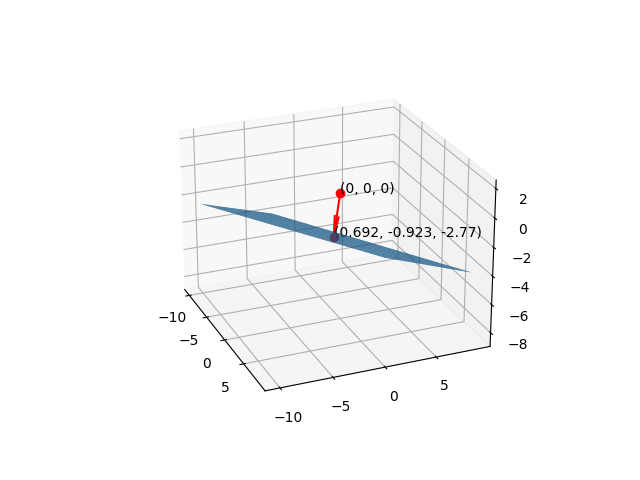
\includegraphics[width=\linewidth]{Graph_3D}
		\caption{Graph of the given plane}
	\end{figure}


\end{document}